% !Mode:: "TeX:UTF-8"
\chapter{实验分析}

\section{实验过程}

该文选择 WSLT 2017 De-En\upcite{iwslt} 和 WMT 2014 De-En\upcite{wmt} 作为机器翻译数据集,XSUM\upcite{xsum} 和 CNN/DailyMail\upcite{cnn}作为摘要生成数据集。

在模型的选择方面,使用 mT5-large and small\upcite{xue2021mt5} 作为机器翻译模型,使用 T5-large and small \upcite{raffel2023exploring} 作为摘要生成模型。大小模型相差约 20 倍。

该文在对预先训练好的大模型进行 50 万步的微调,从而得到基准的大模型。为了实现预测对齐,先使用完成微调的大型模型从输入数据集 $\mathcal{X}_{\text {cal }}=\left\{x^{(i)}\right\}$ 生成输出序列 $\mathcal{Y}_{\text {cal }}=\left\{y^{(i)}\right\}$,创建校准数据集。然后,使用校准数据集 $\left(x_{\text {cal }}, y_{\text {cal }}\right) \in\left(\mathcal{X}_{\text {cal }}, \mathcal{Y}_{\text {cal }}\right)$ 对小模型进行微调。

推理评估在 GCP n1-standard-4 实例的单个 NVIDIA T4 GPU 上进行。该文对不同的 Fallback 和 Rollback 阈值进行了测试,并分别使用或关闭预测对齐,探究生成质量和延迟的权衡。

\section{实验结果}

通过调整 Fallback 和 Rollback 阈值和是否使用预测对齐,研究文本生成质量与推理速度的关系,主要结果如图~\ref{result} 和表~\ref{result_table} 所示。图表中给出了 Vanilla Inference 基准数据。在消融研究中,分别去除 Fallback 和 Rollback 部分,验证 BiLD 的有效性。

\begin{figure}[htbp]
    \centering
    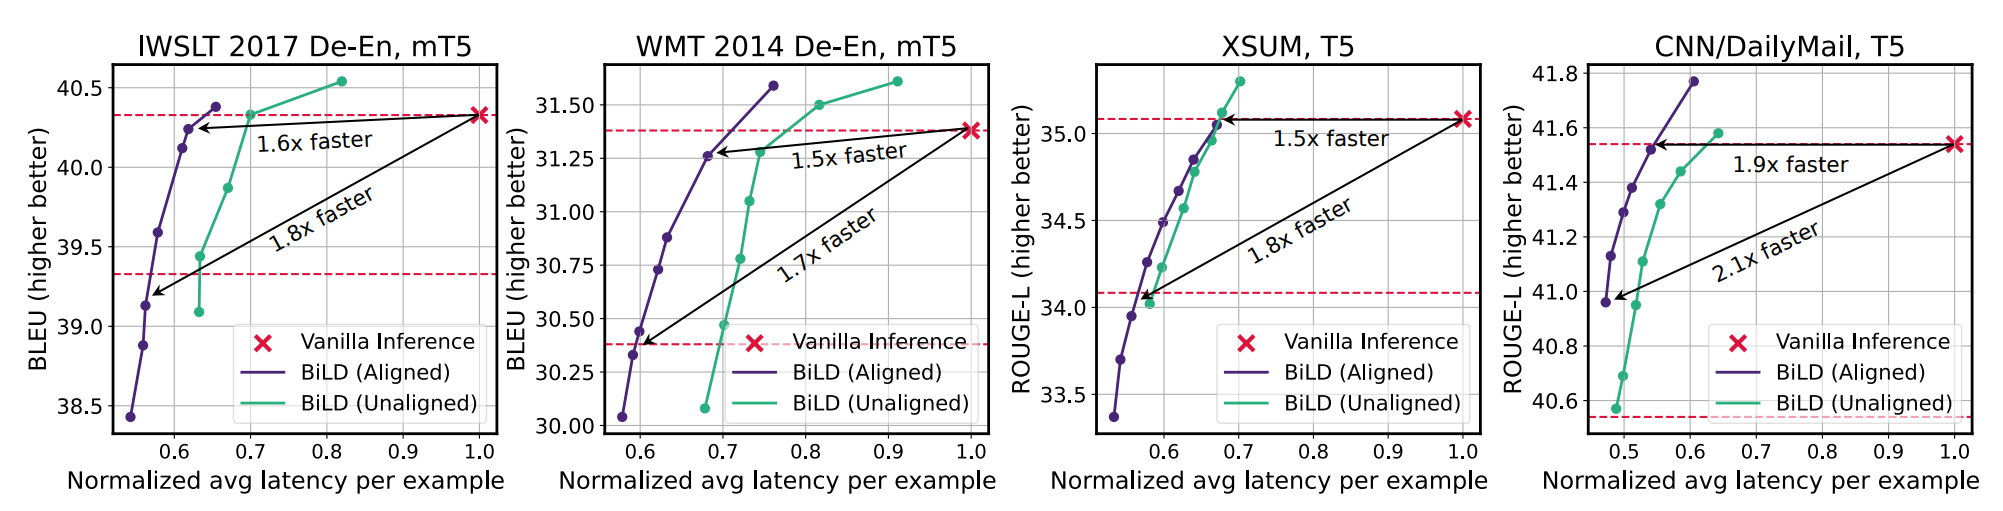
\includegraphics[width=0.9\textwidth]{result.png}
    \caption{实验数据:紫线和绿线分别代表是否开启预测对齐的BiLD,两条红线指示基准推理分数和其低 1 分的位置}
    \label{result}
\end{figure}

\begin{table}[htbp]
    \centering
    \caption{实验数据总结}
    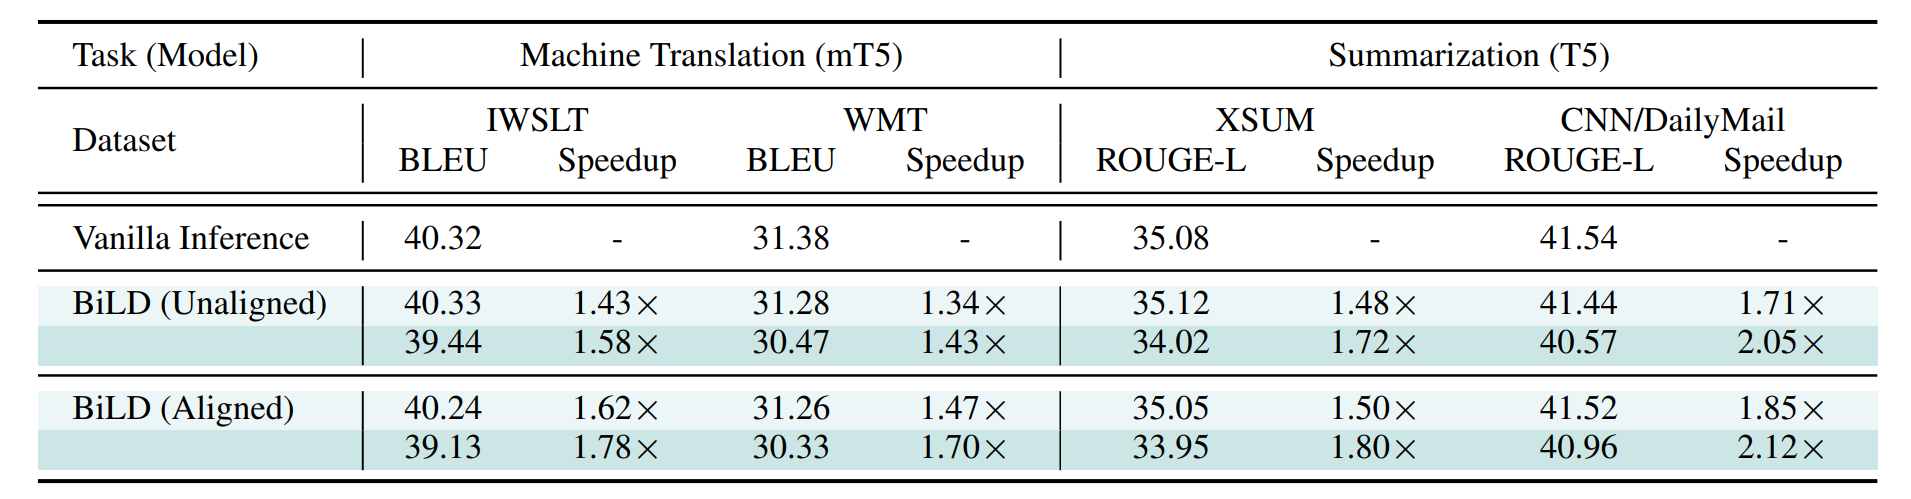
\includegraphics[width=0.9\textwidth]{result_table.png}
    \label{result_table}
\end{table}
在不进行预测对齐时, BiLD 相对所有基准测试平均提速至 $1.5\sim 2.0$ 倍。未对齐的 BiLD 是一种纯粹的即插即用解决方案,除了独立准备小型模型外,不需要额外的工作。

对齐的 BiLD 比未对齐的 BiLD 有了进一步改进,提速为 $1.6\sim 2.1$ 倍。结果还表明,在允许高延迟时(仍比基准模型快),未对齐和已对齐的 BiLD 都优于基准分数,这可以归因于使用两种不同模型的集合效应\upcite{matsubara2022ensemble}。

\section{消融研究}

分别取消 Rollback 和 Fallback ,研究 BiLD 有效性。在取消 Rollback 策略时,使用与主实验相同的 Fallback 阈值;取消 Fallback 策略时,使用与主实验相同的 Rollback 阈值,并在小模型执行固定数量的预测后将控制权移交给大模型,与 \upcite{chen2023accelerating} 类似。

\begin{figure}[htbp]
    \centering
    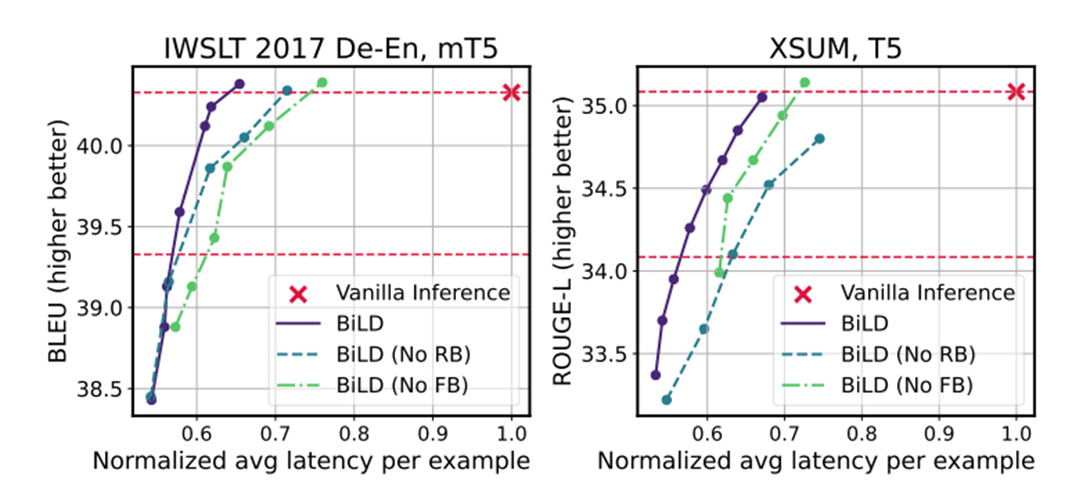
\includegraphics[width=0.9\textwidth]{ablation.png}
    \caption{
        消融实验:分别去除 Rollback 和 Fallback,与完整的 BiLD 和基准模型对比
    }
    \label{ablation}
\end{figure}

图~\ref{ablation} 消融实验数据表明,Rollback 策略能提升质量,大模型 Rollback 纠正小模型的错误预测至关重要。尽管撤销标记会导致重复计算开销,但生成质量的提高更加显著。同样,取消 Fallback 策略并在生成一定数量的标记后定期将控制权移交给大型模型,也会导致性能明显下降。综上所述,BiLD 的 Fallback 和 Rollback 策略都是有效的。
